\chapter{التقنيات المخبرية \texorpdfstring{\babelsublr{(1)}}{(1)}: السلامة والقياس والفصل}\label{ch:b1:lab-techniques-1}

يعيد طالبان \omterm{def:b1:crystals-metals:crystal}{بلورة} الدفعة نفسها من الأسبرين ويقيسان درجة
انصهارها على المنصة الساخنة نفسها. فيقرأ أحدهما \qty{134}{\celsius}،
والآخر \qty{136}{\celsius}. هل يختلفان؟ وهل الناتج نقي؟ لا يمكن الإجابة عن
أي من السؤالين بالعددين وحدهما: فالقياس لا قيمة له إلا
مع عدم يقينه، والمقارنة لا قيمة لها إلا مع
قاعدة. يجمع هذا الفصل الأخير الجانب العملي من السنة: كيف
تُقرأ \omterm{def:b1:lab-techniques-1:hazard}{أخطار} ما على طاولة العمل، وكيف تُذكر قيمة مقيسة
وعدم يقينها وتُقارن بقيمة أخرى، وكيف تفصل العمليات الكلاسيكية
في المختبر العضوي --- الاستخلاص، والترشيح،
\omterm{def:b1:lab-techniques-1:recrystallisation}{وإعادة التبلور}، والتقطير --- ناتجًا عما
يحيط به، ثم تتحقق من نقاوته.

\begin{recall}
\omterm{def:b1:precipitation:solubility}{الذوبانية} والامتزاج انطلاقًا من القوى بين الجزيئية، \omterm{def:b1:intermolecular-forces-solvents:solvent-classes}{والمذيبات القطبية} واللاقطبية
(\cref{ch:b1:intermolecular-forces-solvents})؛ والسحاحات والماصّات
\omterm{def:b1:titration-methods:titration}{ونقطة نهاية} \omterm{def:b1:titration-methods:titration}{المعايرة} (\cref{ch:b1:titration-methods}). وقد قدّم
المجلد المدرسي (الصف العاشر) الاستخلاص سائل--سائل،
\omterm{def:b1:lab-techniques-1:recrystallisation}{وإعادة التبلور}، وكروماتوغرافيا الطبقة الرقيقة \omterm{def:b1:extent-q-and-k:fractional-extent}{ومردود} التخليق؛
وهنا تُعطى أرقامها.
\end{recall}

\begin{omfigure}
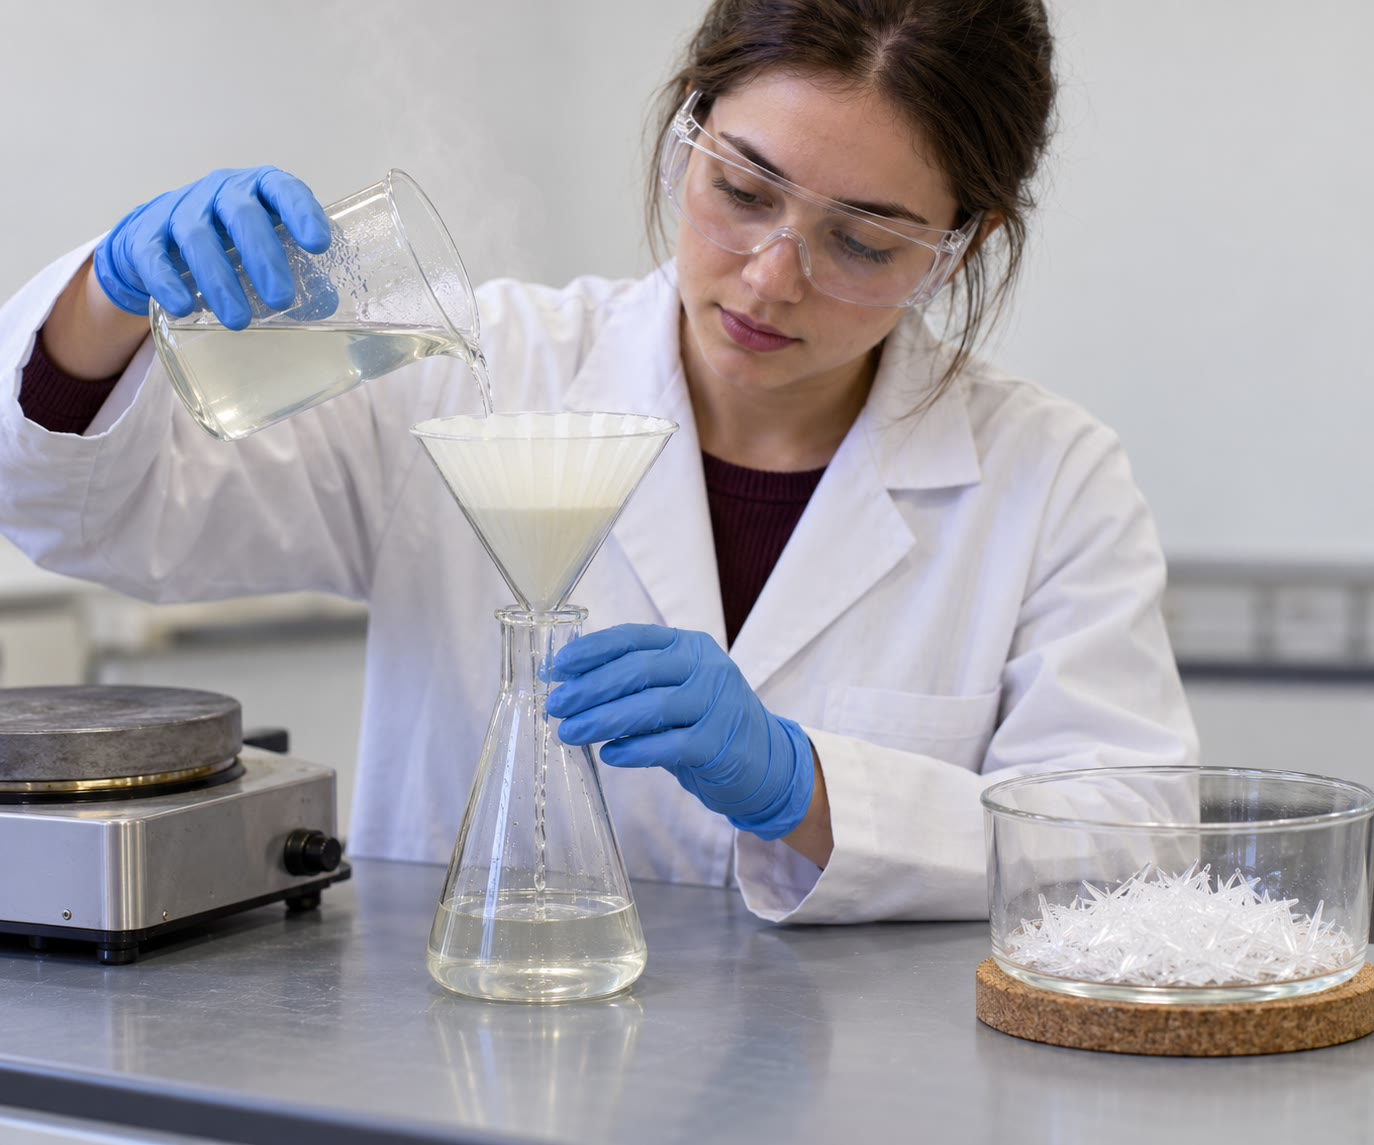
\includegraphics[width=0.5\linewidth]{images/book2/ai/b1-29-recrystallisation.jpg}

{\small ترشيح على الساخن أثناء \omterm{def:b1:lab-techniques-1:recrystallisation}{إعادة تبلور}: نظارات واقية، وقفازات
ومئزر مخبري؛ يمر المحلول الساخن عبر ورقة ترشيح مطوية، التي
تحتجز الشوائب غير الذوابة. وتنتظر إبر ناتج أُعيدت بلورته
في الطبق على اليمين.}
\end{omfigure}

\section{الأخطار وبطاقاتها}

\begin{definition}[الخطر والخطورة]\label{def:b1:lab-techniques-1:hazard}
\emph{الخطر}\index{خطر} هو الخاصية الذاتية لمادة (أو
لوضع ما) التي يمكن أن تُحدث ضررًا: قابلية الاشتعال، والتآكل،
والسمية. و\emph{الخطورة}\index{خطورة} هي احتمال وقوع الضرر فعلًا،
وشدته، في ظروف الاستعمال المعطاة: وهي تتعلق
بالخطر وبالتعرّض (الكمية، والتركيز، والمدة، والطريق،
والوقاية).
\end{definition}

لا يمكن تغيير \omterm{def:b1:lab-techniques-1:hazard}{الخطر} دون تغيير المادة؛ أما \omterm{def:b1:lab-techniques-1:hazard}{الخطورة} فتُخفض
بالعمل على التعرّض: كمية أصغر، أو محلول أكثر تخفيفًا،
أو خزانة غازات، أو قفازات ونظارات، أو كاشف أقل خطرًا
للمهمة نفسها.

\begin{definition}[وسم GHS]\label{def:b1:lab-techniques-1:ghs}
تتبع بطاقات المواد الكيميائية النظام المنسَّق عالميًا (GHS).
\begin{itemize}
  \item \emph{الرسم التحذيري للخطر}\index{رسم تحذيري للخطر} رمز أسود
        على معيّن أبيض بإطار أحمر؛ وهي تسعة، من \texttt{GHS01}
        إلى \texttt{GHS09}.
  \item \emph{كلمة التنبيه}\index{كلمة التنبيه} هي \emph{خطر} لفئات
        \omterm{def:b1:lab-techniques-1:hazard}{الخطر} الأشد و\emph{تحذير} للأقل
        شدة؛ ولا تحمل البطاقة إلا كلمة واحدة، هي الأشد.
  \item \emph{بيان الخطر}\index{بيان الخطر} عبارة معيارية،
        مرمّزة بالحرف H متبوعًا بثلاثة أرقام، تصف خطرًا:
        H2xx \omterm{def:b1:lab-techniques-1:hazard}{الأخطار} الفيزيائية، وH3xx \omterm{def:b1:lab-techniques-1:hazard}{الأخطار} الصحية، وH4xx \omterm{def:b1:lab-techniques-1:hazard}{الأخطار}
        البيئية.
  \item \emph{البيان الاحتياطي}\index{بيان احتياطي}،
        المرمّز بالحرف P وثلاثة أرقام، يعطي تدبيرًا يُتخذ: P1xx عام،
        وP2xx الوقاية، وP3xx الاستجابة، وP4xx التخزين، وP5xx التخلص.
  \item \emph{صحيفة بيانات السلامة}\index{صحيفة بيانات السلامة} هي
        الوثيقة التي يقدمها المورّد مع المنتج، في أقسام
        معيارية: التعريف، \omterm{def:b1:lab-techniques-1:hazard}{والأخطار}، والتركيب، والإسعافات الأولية،
        ومكافحة الحريق، والتداول والتخزين، وضبط التعرّض
        والوقاية، والخواص الفيزيائية والكيميائية، والثبات، والسمية،
        والتخلص والنقل.
\end{itemize}
\end{definition}

\begin{omfigure}
\setlength{\tabcolsep}{5pt}
\begin{tabular}{ccccc}
\begin{tabular}[t]{@{}c@{}}\ghs[1.25cm]{GHS01}\\[2pt]\footnotesize GHS01\\\footnotesize متفجر\end{tabular} &
\begin{tabular}[t]{@{}c@{}}\ghs[1.25cm]{GHS02}\\[2pt]\footnotesize GHS02\\\footnotesize قابل للاشتعال\end{tabular} &
\begin{tabular}[t]{@{}c@{}}\ghs[1.25cm]{GHS03}\\[2pt]\footnotesize GHS03\\\footnotesize مؤكسد\end{tabular} &
\begin{tabular}[t]{@{}c@{}}\ghs[1.25cm]{GHS04}\\[2pt]\footnotesize GHS04\\\footnotesize غاز تحت الضغط\end{tabular} &
\begin{tabular}[t]{@{}c@{}}\ghs[1.25cm]{GHS05}\\[2pt]\footnotesize GHS05\\\footnotesize أكّال\end{tabular} \\[8pt]
\begin{tabular}[t]{@{}c@{}}\ghs[1.25cm]{GHS06}\\[2pt]\footnotesize GHS06\\\footnotesize سمية حادة\end{tabular} &
\begin{tabular}[t]{@{}c@{}}\ghs[1.25cm]{GHS07}\\[2pt]\footnotesize GHS07\\\footnotesize ضار، مهيّج\end{tabular} &
\begin{tabular}[t]{@{}c@{}}\ghs[1.25cm]{GHS08}\\[2pt]\footnotesize GHS08\\\footnotesize خطر صحي\end{tabular} &
\begin{tabular}[t]{@{}c@{}}\ghs[1.25cm]{GHS09}\\[2pt]\footnotesize GHS09\\\footnotesize البيئة\end{tabular} & \\
\end{tabular}

\smallskip
{\small الرسوم التحذيرية التسعة في GHS: قنبلة متفجرة، ولهب، ولهب فوق دائرة،
وأسطوانة غاز، وتآكل، وجمجمة وعظمتان متقاطعتان، وعلامة تعجب، وخطر
صحي (آثار طويلة الأمد: السرطان، والطفرات، والإنجاب، وتحسس
المسالك التنفسية، والاستنشاق الرئوي) والبيئة.}
% ledger: ghspic:GHS01, ghspic:GHS02, ghspic:GHS03, ghspic:GHS04,
% ghspic:GHS05, ghspic:GHS06, ghspic:GHS07, ghspic:GHS08, ghspic:GHS09
\end{omfigure}

\begin{example}[قراءة بطاقة الإيثانول]
تحمل قارورة الإيثانول الرسمين التحذيريين GHS02 وGHS07، \omterm{def:b1:lab-techniques-1:ghs}{وكلمة
التنبيه} \emph{خطر}، والبيانين H225 (سائل وبخار شديدا الاشتعال، وهو
\omterm{def:b1:lab-techniques-1:hazard}{خطر} فيزيائي تستدعي فئته \emph{خطر}) وH319
(يسبب تهيجًا شديدًا للعين، وهو خطر صحي، يستدعي وحده \emph{تحذير}).
ومن بياناته الاحتياطية P210 (يُحفظ بعيدًا عن الحرارة والشرر
واللهب المكشوف؛ ممنوع التدخين)، وP233 (يُحفظ الوعاء محكم الإغلاق)، وP280
(ارتدِ القفازات ووقاية العينين)، و\babelsublr{P305+P351+P338} (في حالة دخوله العينين: اشطفهما
بحذر بالماء لعدة دقائق، وانزع العدسات اللاصقة، وواصل
الشطف) و\babelsublr{P403+P235} (يُخزَّن في مكان جيد التهوية، ويُحفظ باردًا).
والعواقب العملية: لا لهب على طاولة العمل حيث يُستعمل الإيثانول،
ونظارات، وقارورة مغلقة.
\end{example}
% ledger: ghs:ethanol, hstat:H225, hstat:H319, pstat:P210, pstat:P233,
% pstat:P280, pstat:P305+P351+P338, pstat:P403+P235

\begin{method}[تحضير حصة عملية من صحائف بيانات السلامة]\label{met:b1:lab-techniques-1:read-sds}
لكل مادة مستعملة أو متكوّنة:
\begin{enumerate}
  \item اقرأ رسومها التحذيرية، \omterm{def:b1:lab-techniques-1:ghs}{وكلمة التنبيه} وبيانات H (القسم 2 من
        الصحيفة)، ودوّن \omterm{def:b1:lab-techniques-1:hazard}{الأخطار} الفيزيائية (الحريق، والضغط،
        والتفاعلية) بمعزل عن \omterm{def:b1:lab-techniques-1:hazard}{الأخطار} الصحية والبيئية؛
  \item قدّر التعرّض لكل عملية (الوزن، والتسخين، والنقل، والترشيح):
        الكمية، والحالة (فالسائل المتطاير أو
        المسحوق الناعم يبلغ الرئتين)، والمدة؛
  \item اختر التدابير: الاستعاضة بكاشف أقل خطرًا،
        وتصغير السلّم، وخزانة الغازات، ثم الوقاية الشخصية (بيانات
        P2xx)؛
  \item خطّط للاستجابة لحادث (P3xx: العينان، والجلد، والبلع،
        والحريق) ولوجهة كل نفاية (P5xx).
\end{enumerate}
\end{method}

\begin{inthelab}[النفايات]
لا يذهب شيء إلى المغسلة افتراضيًا. فتُجمع المذيبات العضوية في
وعاءين، المهلجنة (ثنائي كلورو الميثان، والكلوروفورم)
وغير المهلجنة (الإيثانول، والبروبانون، والهكسان الحلقي، وإيثانوات الإيثيل)، لأنها
تُعالج بطرق مختلفة؛ وتُعادل المحاليل المائية الحمضية والقاعدية
قبل التخلص منها؛ ولمحاليل أيونات الفلزات الثقيلة (الكروم،
والنحاس، والفضة) أوعيتها الخاصة؛ ويُحفظ الزجاج المكسور والأجسام الصلبة
الملوثة بمعزل عن القمامة العادية. والبيان P273، «تجنَّب
إطلاقه في البيئة»، على البطاقة يذكّر بأن وعاء النفايات،
لا البالوعة، هو نهاية التجربة.
% ledger: pstat:P273
\end{inthelab}

\section{القياس وعدم اليقين}

القيمة المقيسة ليست أبدًا القيمة الدقيقة للمقدار المقيس: أعد
القياس فتتغير النتيجة قليلًا؛ واقرأ التدريج فيكون
الرقم الأخير تخمينًا. ويبيّن \omterm{def:b1:lab-techniques-1:uncertainty}{عدم اليقين} إلى أي حد يمكن معقولًا أن تبعد
القيمة الحقيقية عن القيمة المقيسة.

\begin{definition}[عدم يقين القياس]\label{def:b1:lab-techniques-1:uncertainty}
\begin{itemize}
  \item \emph{عدم يقين القياس}\index{عدم يقين القياس}
        وسيط يميّز تشتت القيم
        التي يمكن معقولًا أن تُنسب إلى المقدار المقيس.
  \item \emph{عدم اليقين المعياري}\index{عدم اليقين المعياري} $u(x)$
        هو عدم اليقين ذاك معبَّرًا عنه بانحراف معياري.
  \item \emph{التقييم من النوع A}\index{تقييم من النوع A} يعطي $u$ من
        التحليل الإحصائي لسلسلة من القياسات المكررة؛
        و\emph{التقييم من النوع B}\index{تقييم من النوع B} يعطيه بأي
        وسيلة أخرى: تدريج أداة، أو التفاوت الذي يذكره
        صانعها، أو شهادة معايرة، أو عدد أرقام
        قيمة مجدولة.
  \item \emph{عدم اليقين الموسَّع}\index{عدم اليقين الموسع}
        $U = k\,u$ هو عدم اليقين المعياري مضروبًا في معامل
        تغطية $k$، يساوي عادةً $k = 2$؛ وفي التوزيع الطبيعي يحتوي
        المجال $x \pm 2u$ القيمة الحقيقية باحتمال يبلغ
        نحو \qty{95}{\percent}.
  \item \emph{عدم اليقين النسبي}\index{عدم اليقين النسبي} هو
        $u(x)/|x|$، ويُعطى غالبًا بالنسبة المئوية.
\end{itemize}
\end{definition}

\begin{proposition}[التقييم من النوع A]\label{prop:b1:lab-techniques-1:type-a}
إذا أُجري $n$ قياسًا مستقلًا $x_1, \dots, x_n$ للمقدار نفسه،
فأفضل تقدير هو متوسطها $\bar x$؛ والانحراف المعياري
التجريبي هو
\[
  s = \sqrt{\frac{1}{n-1} \sum_{i=1}^{n} (x_i - \bar x)^2},
\]
ويكون \omterm{def:b1:lab-techniques-1:uncertainty}{عدم اليقين المعياري} للمتوسط $u(\bar x) = s/\sqrt{n}$.
\end{proposition}
\begin{proof}[\omnameProof]
\emph{نقبله في هذا المستوى}؛ أما إحصاء القياسات المكررة،
ومنه معامل ستيودنت المستعمل حين يكون $n$ صغيرًا، فيُعالج في
مجلد السنة الثانية.
\end{proof}

\begin{omfigure}
\begin{tikzpicture}
\begin{axis}[width=7.4cm, height=5cm, xlabel={\foreignlanguage{arabic}{حجم نقطة النهاية بالوحدة \unit{mL}}},
  ylabel={عدد القراءات}, ymin=0, ymax=8.5, xmin=12.2, xmax=12.7,
  xtick={12.2,12.3,12.4,12.5,12.6,12.7},
  xticklabel style={/pgf/number format/fixed, /pgf/number format/precision=1},
  axis lines=left, every axis plot/.append style={line join=round}]
  \addplot[ybar, bar width=0.045, fill=omDef!35, draw=omDef!80!black]
    table[x=V, y=count] {figdata/out/bachelor-1-type-a-uncertainty-a.dat};
  \addplot[omThm, thick, smooth]
    table[x=V, y=g] {figdata/out/bachelor-1-type-a-uncertainty-b.dat};
  \draw[omProp, thick, <->] (axis cs:12.384,7.6) -- (axis cs:12.526,7.6);
  \node[omProp, font=\small, above] at (axis cs:12.455,7.6) {$\bar V \pm s$};
\end{axis}
\end{tikzpicture}\hspace{0.6cm}%
\begin{tikzpicture}
\begin{axis}[width=5.6cm, height=5cm, xlabel={\babelsublr{$x - x_0$}}, ylabel={كثافة الاحتمال},
  ymin=0, ymax=0.8, xmin=-1.6, xmax=1.6, xtick={-1,0,1},
  xticklabels={$-a$, $0$, $a$}, ytick={0.5}, yticklabels={$\frac{1}{2a}$},
  axis lines=left]
  \addplot[omDef!80!black, thick, fill=omDef!25] coordinates
    {(-1,0) (-1,0.5) (1,0.5) (1,0)} \closedcycle;
  \draw[omProp, thick, <->] (axis cs:-0.577,0.62) -- (axis cs:0.577,0.62);
  \node[omProp, font=\small, above] at (axis cs:0,0.62) {$\pm a/\sqrt3$};
\end{axis}
\end{tikzpicture}

{\small يمينًا: عشرون قراءة \omterm{def:b1:titration-methods:titration}{لنقطة نهاية} \omterm{def:b1:titration-methods:titration}{المعايرة} نفسها (معطيات
توضيحية)، مقروءة بدقة \qty{0.05}{mL}، مع المنحنى الطبيعي ذي المتوسط نفسه
$\bar V = \qty{12.455}{mL}$ والانحراف المعياري نفسه $s = \qty{0.071}{mL}$.
يسارًا: التوزيع المستطيل \omterm{def:b1:lab-techniques-1:uncertainty}{لتقييم من النوع B}، لقيمة لا يُعرف
عنها إلا أنها تقع بين $x_0 - a$ و$x_0 + a$؛ وانحرافها المعياري
$a/\sqrt3$.}
\end{omfigure}

\begin{example}[عشرون نقطة نهاية]
من أجل القراءات العشرين في الشكل، $\bar V = \qty{12.455}{mL}$،
و$s = \qty{0.071}{mL}$ و$u(\bar V) = 0.071/\sqrt{20} = \qty{0.016}{mL}$.
فالقراءة الواحدة غير يقينية بنحو $s$؛ ومتوسط عشرين قراءة بنحو
$s/\sqrt{20}$، أي أقل بأربع مرات ونصف. والنتيجة
$V = \qty{12.46}{mL}$ مع $U = 2u = \qty{0.03}{mL}$.
\end{example}

\begin{proposition}[التقييم من النوع B لتوزيع مستطيل]\label{prop:b1:lab-techniques-1:type-b}
إذا كان كل ما يُعرف عن مقدار أنه يقع، باحتمال
متساوٍ، في أي موضع بين $x_0 - a$ و$x_0 + a$، فإن عدم يقينه
المعياري هو
\[
  u = \frac{a}{\sqrt3}.
\]
\end{proposition}
\begin{proof}
كثافة الاحتمال $1/(2a)$ على $[x_0 - a, x_0 + a]$ ومنعدمة
خارجه؛ ومتوسطها $x_0$ بالتناظر وتباينها هو
\[
  u^2 = \int_{x_0-a}^{x_0+a} (x - x_0)^2 \frac{\mathrm{d}x}{2a}
      = \frac{1}{2a} \left[\frac{t^3}{3}\right]_{-a}^{a}
      = \frac{1}{2a}\cdot\frac{2a^3}{3} = \frac{a^2}{3}. \qedhere
\]
\end{proof}

\begin{example}[قراءة وتفاوت]
سحاحة مدرّجة كل \qty{0.1}{mL} تُقرأ بدقة نصف تدريجة: فتقع
القراءة ضمن $\pm\qty{0.05}{mL}$ من القيمة المدوّنة، ومن ثم
$u = 0.05/\sqrt3 = \qty{0.029}{mL}$. وماصّة \qty{20}{mL} يذكر صانعها
تفاوتًا قدره $\pm\qty{0.03}{mL}$ تعطي حجمها مع
$u = 0.03/\sqrt3 = \qty{0.017}{mL}$. والقيمة المجدولة المعطاة على هيئة
\qty{135}{\celsius} معروفة ضمن $\pm\qty{0.5}{\celsius}$: $u = \qty{0.29}{\celsius}$.
\end{example}

\begin{proposition}[تركيب أوجه عدم اليقين]\label{prop:b1:lab-techniques-1:combine}
من أجل مقادير مستقلة: إذا كان $y = x_1 + x_2$ أو $y = x_1 - x_2$، فإن
$u(y)^2 = u(x_1)^2 + u(x_2)^2$؛ وإذا كان $y = x_1 x_2$ أو $y = x_1/x_2$، فإن
\[
  \left(\frac{u(y)}{y}\right)^2 = \left(\frac{u(x_1)}{x_1}\right)^2
  + \left(\frac{u(x_2)}{x_2}\right)^2 .
\]
وتتركب المصادر المتعددة \omterm{def:b1:lab-techniques-1:uncertainty}{لعدم اليقين} في المقدار نفسه (جزء من النوع A
وأجزاء من النوع B) بالطريقة نفسها، مجموعًا للمربعات.
\end{proposition}
\admitted

المربعات، لا أوجه \omterm{def:b1:lab-techniques-1:uncertainty}{عدم اليقين} نفسها، هي التي تُجمع: فخطآن مستقلان
نادرًا ما يدفعان في الاتجاه نفسه بكامل قيمتهما. والحجم المعاير
فرق بين قراءتين للسحاحة، فيكون \omterm{def:b1:lab-techniques-1:uncertainty}{عدم يقين} قراءته
$\sqrt2 \times \qty{0.029}{mL} = \qty{0.041}{mL}$؛ ويطغى مصدر كبير واحد
\omterm{def:b1:lab-techniques-1:uncertainty}{لعدم اليقين} على المصادر الأخرى، وهناك ينبغي التماس
التحسين. أما القاعدة العامة، بالمشتقات الجزئية، فمكانها
مجلد السنة الثانية.

\begin{method}[إعلان نتيجة]\label{met:b1:lab-techniques-1:report-result}
\begin{enumerate}
  \item اذكر مصادر \omterm{def:b1:lab-techniques-1:uncertainty}{عدم اليقين}؛ وقيّم كلًّا منها على هيئة \omterm{def:b1:lab-techniques-1:uncertainty}{عدم يقين
        معياري} (من النوع A انطلاقًا من سلسلة، ومن النوع B على هيئة $a/\sqrt3$ انطلاقًا من
        نصف عرض).
  \item ركّبها مجموعًا للمربعات (\cref{prop:b1:lab-techniques-1:combine}).
  \item أعطِ \omterm{def:b1:lab-techniques-1:uncertainty}{عدم اليقين الموسَّع} $U = 2u$ برقم معنوي واحد أو اثنين،
        وقرّب القيمة إلى المنزلة العشرية
        نفسها: $x = (\text{القيمة} \pm U)$ الوحدة، $k = 2$.
\end{enumerate}
\end{method}

\begin{definition}[الانحراف المطبَّع]\label{def:b1:lab-techniques-1:z-score}
\emph{الانحراف المطبَّع}\index{انحراف مطبع} (أو القيمة $z$)
بين قيمتين مستقلتين $x_1$ و$x_2$ للمقدار نفسه،
عدما يقينهما المعياريان $u_1$ و$u_2$، هو
\[
  z = \frac{|x_1 - x_2|}{\sqrt{u_1^2 + u_2^2}} .
\]
وتُعدّ القيمتان متوافقتين حين يكون $z \le 2$؛ وتكون القيمة المقيسة
متوافقة مع قيمة مرجعية بالشرط نفسه.
\end{definition}

\begin{example}[الطالبان]
درجتا الانصهار في مطلع الفصل، \qty{134}{\celsius}
و\qty{136}{\celsius}، حُصل على كل منهما \omterm{def:b1:lab-techniques-1:uncertainty}{بعدم يقين معياري} قدره
\qty{0.8}{\celsius} (القراءة ومعايرة المنصة). عندئذ
$z = 2/\sqrt{0.8^2 + 0.8^2} = 1.8 \le 2$: فالطالبان متفقان. ومتوسطهما،
\qty{135}{\celsius}، متوافق أيضًا مع درجة الانصهار المجدولة
للأسبرين، \qty{135}{\celsius} بتسخين سريع. والقيمة المجدولة
المعطاة إلى الوحدة لها $u = 0.5/\sqrt3 = \qty{0.29}{\celsius}$، فتكون القراءة
الواحدة ذات $u = \qty{0.8}{\celsius}$ متوافقة معها ما دامت تقع
ضمن $2\sqrt{0.8^2 + 0.29^2} = \qty{1.7}{\celsius}$ منها: فالقراءة
التي تقل عن نحو \qty{133}{\celsius} كانت ستدل على ناتج غير نقي.
\end{example}
% ledger: mp:aspirin

\section{الفصل}

\begin{definition}[معامل التوزيع]\label{def:b1:lab-techniques-1:partition-coefficient}
حين يتوزع مذاب A، عند التوازن، بين مذيبين
غير ممتزجين، \omterm{def:b1:extent-q-and-k:system}{طور} عضوي \omterm{def:b1:extent-q-and-k:system}{وطور} مائي، فإن نسبة
تركيزيه
\[
  K = \frac{[\mathrm{A}]_{\mathrm{org}}}{[\mathrm{A}]_{\mathrm{aq}}}
\]
تكون، في المحاليل المخففة عند درجة حرارة معطاة، ثابتًا: هو
\emph{معامل التوزيع}\index{معامل التوزيع} للمادة A بين
المذيبين.
\end{definition}

\begin{proposition}[عدة استخلاصات خير من استخلاص واحد]\label{prop:b1:lab-techniques-1:multiple-extractions}
يُستخلص حجم $V_a$ من محلول مائي $n$ مرة، كل مرة بحجم
جديد $V_o$ من مذيب عضوي. فيكون كسر A الباقي في
\omterm{def:b1:extent-q-and-k:system}{الطور} المائي
\[
  f_n = \left(1 + K \frac{V_o}{V_a}\right)^{-n}.
\]
ومن أجل حجم كلي ثابت من المذيب، تستخلص $n$ أجزاء صغيرة أكثر مما يستخلصه
جزء واحد كبير.
\end{proposition}
\begin{proof}
لتكن $m$ كمية A في \omterm{def:b1:extent-q-and-k:system}{الطور} المائي قبل استخلاص ما،
و$m'$ بعده. عند التوازن يحتوي \omterm{def:b1:extent-q-and-k:system}{الطور} العضوي $m - m'$،
و$K = \dfrac{(m - m')/V_o}{m'/V_a}$، ومن ثم $m - m' = K\dfrac{V_o}{V_a} m'$
و$m' = m\big/\bigl(1 + K V_o/V_a\bigr)$. وكل استخلاص يضرب
الكمية الباقية في العامل نفسه؛ وبعد $n$ منها، يكون $f_n$ القوة
ذات الأس $n$ لذلك العامل. ومع حجم كلي $V$ مقسَّم إلى $n$ جزءًا حجم كل منها $V/n$،
$\ln f_n = -n \ln(1 + KV/(nV_a))$؛ ولأن $\ln(1+t)/t$ تتناقص مع $t$،
فإن $n \ln(1 + t/n)$ تتزايد مع $n$ من أجل $t = KV/V_a > 0$، و$f_n$
تتناقص، نحو النهاية $\mathrm{e}^{-KV/V_a}$.
\end{proof}

\begin{example}[جزء واحد أم ثلاثة]
مذاب له $K = 4$ يُستخلص من \qty{100}{mL} من الماء بمقدار
\qty{60}{mL} من إيثانوات الإيثيل. بجزء واحد،
$f_1 = 1/(1 + 4 \times 0.6) = 0.29$: يُستخلص \qty{71}{\percent}.
وبثلاثة أجزاء من \qty{20}{mL}، $f_3 = (1 + 4 \times 0.2)^{-3} = 0.17$:
\qty{83}{\percent}. وإيثانوات الإيثيل ($\rho = \qty{0.90}{g/cm^3}$) هي
الطبقة العليا في قمع الفصل؛ أما ثنائي كلورو الميثان
($\rho = \qty{1.33}{g/cm^3}$) فسيكون الطبقة السفلى.
\end{example}
% ledger: rho:ethyl-acetate, rho:CH2Cl2, rho:water

يفصل الترشيح صلبًا عن سائل. فبالجاذبية، عبر ورقة
مطوية في قمع، يحتجز شائبة غير ذوابة من محلول ساخن
يجب ألا يبرد في الطريق (الترشيح على الساخن، كما في الصورة في
مطلع الفصل). وتحت ضغط منخفض، في قمع بوخنر على
دورق ذي ذراع جانبية (كما رُسم في المجلد المدرسي)، يجمع صلبًا
بسرعة ويتركه شبه جاف؛ ويُغسل الصلب على المرشح بقليل
من المذيب البارد.

\begin{definition}[إعادة التبلور]\label{def:b1:lab-techniques-1:recrystallisation}
\emph{إعادة التبلور}\index{إعادة التبلور} تنقّي صلبًا
بإذابته في أدنى كمية من مذيب ساخن يكون فيه شديد الذوبان
ساخنًا وقليل الذوبان باردًا، ثم تركه يتبلور عند التبريد؛
والشوائب إما تبقى ذائبة في المذيب البارد (السائل الأم)
وإما، لكونها غير ذوابة، تُزال مسبقًا بالترشيح على الساخن.
\end{definition}

\begin{method}[إعادة تبلور صلب]\label{met:b1:lab-techniques-1:recrystallise}
\begin{enumerate}
  \item اختر المذيب: الناتج شديد الذوبان ساخنًا وقليل
        الذوبان باردًا، والشوائب الذوابة ذوابة حتى باردًا، ولا
        تفاعل مع الناتج، ودرجة غليان أدنى من درجة انصهار
        الناتج؛ ويمكن ضبط خليط من مذيبين ممتزجين (الإيثانول
        والماء) على الناتج.
  \item أذب الصلب الخام في أدنى كمية من المذيب المغلي، مضافًا
        على دفعات صغيرة، مع الارتداد إذا كان المذيب متطايرًا أو
        قابلًا للاشتعال.
  \item إذا بقيت شائبة غير ذوابة، فرشّح على الساخن.
  \item دع المحلول يبرد ببطء، ثم في الثلج: فالتبريد البطيء يعطي
        بلورات أكبر وأنقى، تحتجز قدرًا أقل من السائل الأم.
  \item رشّح تحت ضغط منخفض، واغسل بقليل من المذيب
        المثلَّج، وجفّف، وزِن؛ وتحقق من النقاوة (درجة الانصهار، TLC).
\end{enumerate}
\end{method}

\begin{example}[ثمن النقاوة]
يذوب الأسبرين في الماء بنحو \qty{3.3}{g/L} عند \qty{25}{\celsius}
و\qty{10}{g/L} عند \qty{37}{\celsius}، وأكثر بكثير قرب درجة
الغليان. فإذا غادر المرشحَ \qty{40}{mL} من السائل الأم و\qty{10}{mL} من ماء الغسل
عند \qty{25}{\celsius}، حملا معهما نحو
$\qty{0.050}{L} \times \qty{3.3}{g/L} = \qty{0.17}{g}$ من الأسبرين، مهما كانت
نقاوته. وكل مليلتر من المذيب يزيد على الحد الأدنى يكلّف من \omterm{def:b1:extent-q-and-k:fractional-extent}{المردود}.
\end{example}
% ledger: sol:aspirin-25, sol:aspirin-37

يُنقّى السائل، أو يُفصل سائلان درجتا غليانهما متباعدتان،
\emph{بالتقطير البسيط}: يُغلى الخليط، ويُكثَّف البخار، الأغنى
بالمكوّن الأكثر تطايرًا، ويُجمع. ودرجة الحرارة عند الذراع
الجانبية هي درجة حرارة البخار الذي يتقطر؛ وما دامت ثابتة، فإن مادة نقية
تعبر. أما السوائل ذات درجات الغليان المتقاربة فتحتاج إلى التقطير التجزيئي، أي إلى عمود
بين الدورق والرأس، ويُعالج بمخططات سائل--بخار
في مجلد السنة الثانية.

\begin{omfigure}
\begin{tikzpicture}[font=\small, scale=0.95]
  \pic[transform shape] at (0,0) {heatingmantle};
  \pic[transform shape] at (0,0) {rbflask={0.45}{orange!25}};
  \foreach \x/\y in {-0.35/0.25,0.05/0.18,0.35/0.3}
    \fill[black!55] (\x,\y) circle (0.06);
  \pic[transform shape] (s) at (0,3.0) {stillhead};
  \pic[transform shape] at ($(s-top)+(0,-0.75)$) {thermometer};
  \pic[transform shape, rotate=-20] (c) at (s-arm) {liebig={3.4}};
  \coordinate (cend) at ($(s-arm)+(-20:3.4)$);
  \pic[transform shape] (a) at (cend) {adapter};
  \pic[transform shape] at ($(a-tip)+(0,-2.4)$) {erlenmeyer={0.22}{orange!12}};
  \draw[<-, omProp, thick] (0.12,3.72) -- (-1.4,4.4) node[left, text=black,
    align=right] {مستودع المحرار\\ بمستوى الذراع الجانبية};
  \draw[<-, omProp, thick] ($(s-arm)+(-20:0.65)+(0.65,0.65)$) -- ++(0.2,0.9)
    node[above, text=black] {خروج الماء};
  \draw[<-, omProp, thick] ($(s-arm)+(-20:2.7)+(-0.2,-0.6)$) -- ++(0.05,-0.9)
    node[below, text=black] {دخول الماء};
  \draw[<-, omProp, thick] (-0.3,0.27) -- (-2.2,0.7) node[left, text=black]
    {حصى الغليان};
  \draw[<-, omProp, thick] (1.35,-0.6) -- (2.3,-1.1) node[right, text=black]
    {سترة التسخين};
  \draw[<-, omProp, thick] ($(a-tip)+(0.75,-2.0)$) -- ++(1.0,0.2)
    node[right, text=black] {المقطَّر};
\end{tikzpicture}

{\small التقطير البسيط. يقرأ المحرار درجة حرارة
البخار الداخل إلى المكثف؛ ويدخل ماء التبريد من الطرف السفلي
للمكثف كي يبقى الغلاف ممتلئًا؛ وتمنع حصى الغليان
الفوران العنيف؛ والجهاز مفتوح على الهواء عند المستقبِل.}
\end{omfigure}

\begin{safety}{\ghs[5mm]{GHS02}}
لا يُغلق جهاز التقطير أبدًا: فالجملة المحكمة الإغلاق تنفجر إذا سُخّنت.
وتُضاف حصى الغليان إلى السائل البارد، لا إلى سائل
ساخن أبدًا (فقد يفور فورًا). ويُجمع المقطَّر القابل للاشتعال بعيدًا
عن أي لهب، والمستقبِل في الثلج إن لزم.
\end{safety}

\section{التعرّف والتحقق من النقاوة}

\begin{definition}[معامل الاحتجاز]\label{def:b1:lab-techniques-1:retention-factor}
في كروماتوغرافيا الطبقة الرقيقة (TLC)، توضع بقعة من العيّنة على
خط الأساس قرب أسفل صفيحة مغطاة \omterm{def:b1:extent-q-and-k:system}{بطور} ثابت
(السيليكا)؛ وتقف الصفيحة في حوض مغلق في قليل من \omterm{def:b1:extent-q-and-k:system}{الطور} المتحرك، الذي
يصعد عبر الطبقة بالخاصية الشعرية ويحمل الأنواع الكيميائية بسرعات
مختلفة. و\emph{معامل الاحتجاز}\index{معامل الاحتجاز} لنوع
كيميائي هو
\[
  R_f = \frac{\text{المسافة التي قطعتها البقعة}}
             {\text{المسافة التي قطعتها جبهة المذيب}},
\]
وكلتاهما مقيسة من خط الأساس؛ $0 \le R_f \le 1$، ومن أجل \omterm{def:b1:extent-q-and-k:system}{طور} ثابت
\omterm{def:b1:extent-q-and-k:system}{وطور} متحرك ودرجة حرارة معطاة فإنه يميّز النوع الكيميائي.
\end{definition}

على السيليكا القطبية، يُحتجز النوع القطبي بقوة أكبر من النوع الأقل
قطبية فيكون له $R_f$ الأصغر؛ \omterm{def:b1:extent-q-and-k:system}{والطور} المتحرك الأكثر قطبية يُبعد كل بقعة
أكثر. وقد يختلف نوعان لهما $R_f$ نفسه على صفيحة واحدة؛
أما قيمتا $R_f$ المختلفتان فتثبتان أنهما مختلفان. والناتج النقي يعطي
بقعة واحدة.

\begin{omfigure}
\begin{tikzpicture}[font=\small, scale=1.7]
  \pic[transform shape] at (0,0) {tlcplate};
  \draw[omDef!80!black, densely dashed, line width=0.5pt] (-0.7,2.7) -- (0.7,2.7);
  \foreach \x in {-0.4,0,0.4} \fill[black!60] (\x,0.4) circle (0.025);
  \fill[omThm!70] (-0.4,{0.4+0.30*2.3}) ellipse (0.09 and 0.06);
  \fill[omDef!70] (0,{0.4+0.65*2.3}) ellipse (0.09 and 0.06);
  \fill[omThm!70] (0.4,{0.4+0.30*2.3}) ellipse (0.09 and 0.06);
  \fill[omDef!70] (0.4,{0.4+0.65*2.3}) ellipse (0.09 and 0.06);
  \node[below] at (-0.4,0) {A}; \node[below] at (0,0) {B};
  \node[below] at (0.4,0) {M};
  \draw[omProp, thick, |<->|] (0.95,0.4) -- (0.95,{0.4+0.65*2.3})
    node[midway, right] {$d_{\mathrm{B}}$};
  \draw[omProp, thick, |<->|] (1.55,0.4) -- (1.55,2.7)
    node[midway, right] {$d_{\mathrm{front}}$};
  \draw[omProp, thick, |<->|] (-0.95,0.4) -- (-0.95,{0.4+0.30*2.3})
    node[midway, left] {$d_{\mathrm{A}}$};
  \node[right, align=left, font=\footnotesize] at (0.75,2.85) {جبهة المذيب};
  \draw[omProp, thick, <-] (-0.6,0.4) -- (-1.2,0.05) node[left, text=black, font=\footnotesize] {خط الأساس};
\end{tikzpicture}

{\small صفيحة TLC بعد التطوير: المرجعان A وB والخليط M،
موضوعة على خط الأساس. $R_f(\mathrm{A}) = d_{\mathrm{A}}/d_{\mathrm{front}}
= 0.30$، $R_f(\mathrm{B}) = 0.65$؛ ويُظهر الخليط البقعتين كلتيهما، على
الارتفاعين نفسيهما.}
\end{omfigure}

\begin{method}[إجراء TLC]\label{met:b1:lab-techniques-1:tlc}
\begin{enumerate}
  \item ارسم خط الأساس بقلم الرصاص على بعد نحو \qty{1}{cm} من الأسفل؛ وضع
        بقعًا صغيرة من محاليل مخففة للعيّنة وللمراجع
        جنبًا إلى جنب.
  \item ضع بضعة مليمترات من \omterm{def:b1:extent-q-and-k:system}{الطور} المتحرك في الحوض (تحت خط الأساس)،
        وأغلقه، ودع الجو يتشبّع؛ ثم أوقف الصفيحة فيه.
  \item أخرج الصفيحة حين تصير الجبهة على بعد نحو \qty{1}{cm} من الأعلى؛
        وعلّم الجبهة فورًا؛ وجفّف.
  \item أظهر البقع عديمة اللون (مصباح فوق بنفسجي على صفيحة متفلورة،
        أو بخار اليود، أو كاشف تلوين)؛ وأحِطها بقلم الرصاص.
  \item قِس المسافات من خط الأساس واحسب كل $R_f$؛
        وقارن العيّنة بالمراجع على الصفيحة نفسها.
\end{enumerate}
\end{method}

\begin{omfigure}
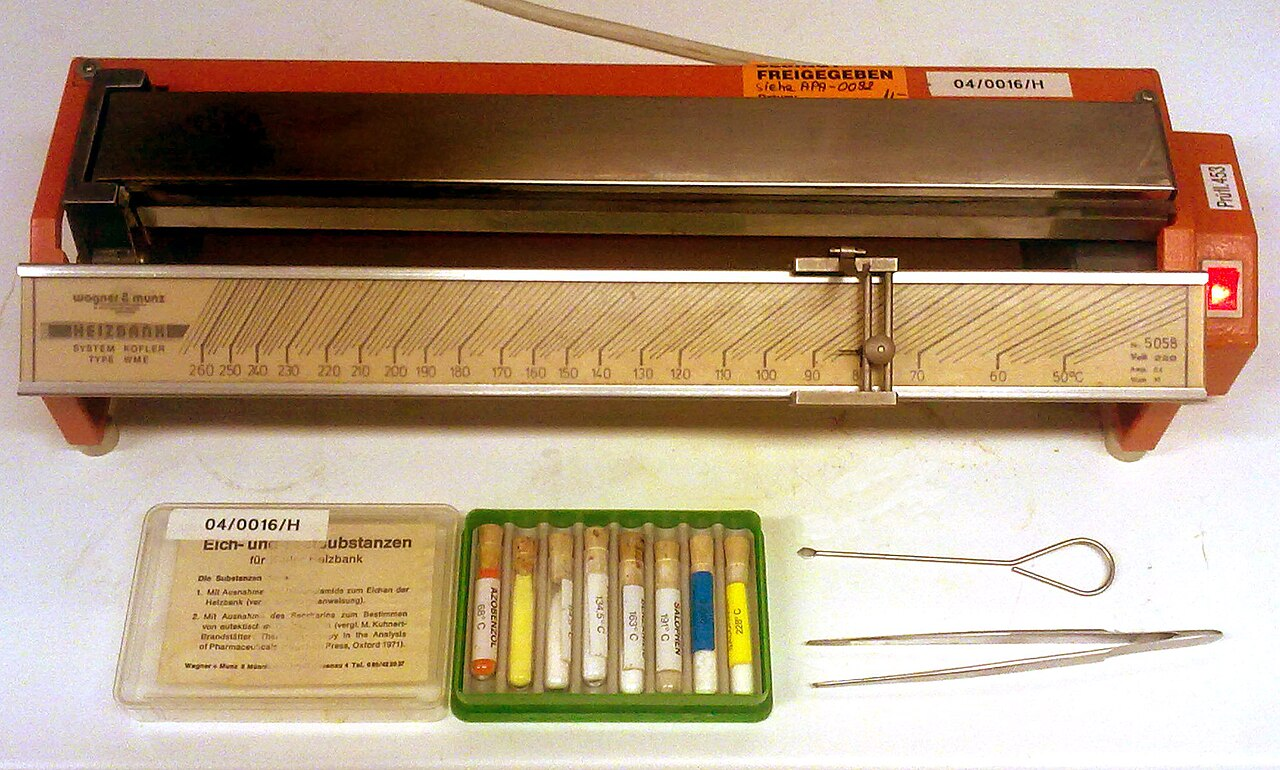
\includegraphics[width=0.62\linewidth]{images/book2/kofler-bench.jpg}

{\small منصة ساخنة (منصة كوفلر): شريط فلزي مسخَّن من أحد طرفيه،
فيه تدرّج في درجة الحرارة على امتداده؛ والصلب المنثور على الشريط
ينصهر بعد خط حاد، يُقرأ على التدريج بالمؤشر. ويحتوي الصندوق
مواد مرجعية معلومة درجة الانصهار، تُستعمل لمعايرته.
الصورة: HBR، CC BY-SA 3.0، ويكيميديا كومنز.}
\end{omfigure}

\begin{method}[قياس درجة انصهار على منصة ساخنة]\label{met:b1:lab-techniques-1:melting-point}
\begin{enumerate}
  \item شغّل المنصة قبل وقت كافٍ: فالتدرّج يحتاج إلى وقت كي
        يستقر.
  \item عايرها بمادة مرجعية نقية تنصهر قرب
        القيمة المتوقعة، منثورة على الشريط؛ واضبط المؤشر بحيث يقرأ
        التدريج درجة انصهارها على الخط.
  \item انثر بضع بلورات من العيّنة الجافة من الطرف البارد
        نحو الطرف الساخن؛ وادفعها ذهابًا وإيابًا بالملعقة
        وضع المؤشر على الحد الذي ينصهر الصلب بعده فورًا.
  \item اقرأ، وكرّر، ونظّف الشريط؛ وخذ متوسط القراءات
        واذكر \omterm{def:b1:lab-techniques-1:uncertainty}{عدم اليقين} (\cref{met:b1:lab-techniques-1:report-result}).
\end{enumerate}
\end{method}

تنصهر المادة البلورية النقية انصهارًا حادًا عند درجة انصهارها؛ أما غير النقية
فتبدأ بالانصهار عند درجة أدنى وتنصهر على مجال من درجات الحرارة، لأن
الشائبة تخفض درجة الحرارة التي يتعايش عندها الصلب والسائل
(والسبب، أي الجهد الكيميائي لمذيب يخفضه
مذاب، موجود في مجلد السنة الثانية). فدرجة الانصهار الأدنى بكثير من
القيمة المجدولة، أو مجال الانصهار العريض، يكشف إذن عن الشوائب؛
والقيمة المتوافقة مع القيمة المجدولة، بمعنى \omterm{def:b1:lab-techniques-1:z-score}{الانحراف المطبَّع}،
تدعم النقاوة دون أن تثبتها.

\begin{inthelab}[معايرة المنصة]
تُختار المراجع بحيث تحيط بالقيمة المتوقعة. فالأسيتانيليد،
الذي ينصهر عند \qty{114.3}{\celsius}، وحمض البنزويك، عند
\qty{122.4}{\celsius}، معياران كلاسيكيان للنواتج التي تنصهر بين
\qty{110}{\celsius} و\qty{130}{\celsius}؛ ومن أجل الأسبرين، يكون المعيار القريب من
\qty{135}{\celsius} أفضل. والأسبرين نفسه يتفكك أثناء انصهاره،
فتتعلق درجة انصهاره المرصودة بسرعة تسخينه: وتعطي الجداول
\qty{135}{\celsius} للتسخين السريع، وهو ما تفعله المنصة.
% ledger: mp:acetanilide, mp:benzoic, mp:aspirin
\end{inthelab}

يُتعرّف السائل، ويُتحقق من نقاوته، \emph{بمعامل
انكساره} $n_D$، وهو نسبة سرعة الضوء في الفراغ إلى سرعته في
السائل، ويُقاس بخط الصوديوم الأصفر D عند درجة حرارة مذكورة
(عادةً \qty{20}{\celsius})، بأربعة أرقام عشرية. فللماء
$n_D = 1.333$، وللإيثانول 1.3611 وللهكسان الحلقي 1.4266 عند \qty{20}{\celsius}.
وينخفض المعامل قليلًا بارتفاع درجة الحرارة، ولذلك يُضبط حرارة
الجهاز بمنظِّم حراري.
% ledger: nD:water, nD:ethanol, nD:cyclohexane

\begin{omfigure}
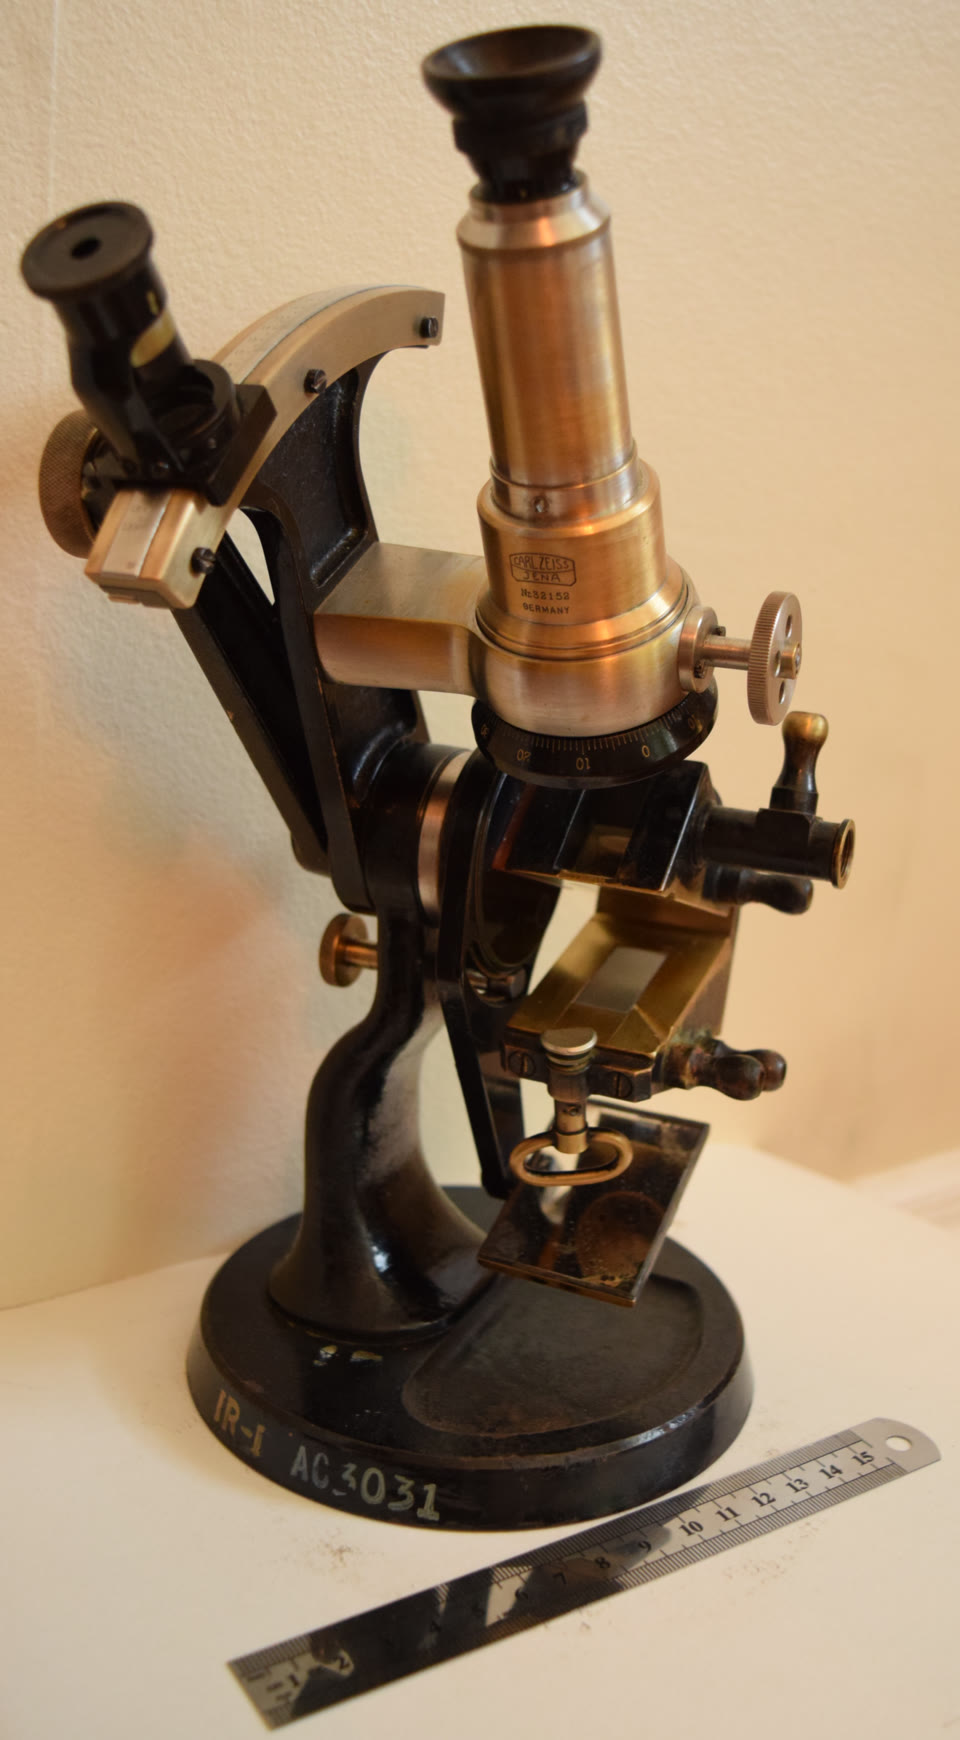
\includegraphics[height=6cm]{images/book2/abbe-refractometer.jpg}

{\small مقياس انكسار آبي: تُفرد قطرة من السائل بين
موشورين؛ وتُظهر العدسة العينية حقلًا نصفه مضيء ونصفه مظلم،
والحد بينهما، إذا وُضع على الشعرتين المتصالبتين، يعطي معامل الانكسار على التدريج.
الصورة: فوريد، CC BY-SA 4.0، ويكيميديا كومنز.}
\end{omfigure}

\section{تمارين}

\begin{exercise}[$\star$]\label{exo:b1:lab-techniques-1:1}
تحمل قارورة البروبانون الرسمين التحذيريين GHS02 وGHS07
والبيانات H225 وH319 وH336. فأي \omterm{def:b1:lab-techniques-1:ghs}{كلمة تنبيه} تحمل؟ وأي
البيانات تصف خطرًا فيزيائيًا، وأيها خطرًا صحيًا؟ واذكر احتياطين
تستدعيهما.
\end{exercise}

\begin{exercise}[$\star$]\label{exo:b1:lab-techniques-1:2}
\omterm{def:b1:lab-techniques-1:hazard}{خطر} أم \omterm{def:b1:lab-techniques-1:hazard}{خطورة}؟ (أ) يسبب حمض الكبريتيك المركّز حروقًا شديدة.
(ب) وزن \qty{50}{mg} من مسحوق سام في خزانة غازات مع
القفازات لا يعرّض المشغّل إلا قليلًا. (ج) يطلق الصوديوم الهيدروجين مع
الماء. (د) المذيب نفسه أشد خطرًا إذا استُعمل ساخنًا في كأس مفتوحة
منه باردًا في قارورة مغلقة.
\end{exercise}

\begin{exercise}[$\star$]\label{exo:b1:lab-techniques-1:3}
على صفيحة TLC تقع جبهة المذيب على ارتفاع \qty{6.0}{cm} فوق خط الأساس؛
وتعطي العيّنة بقعتين عند \qty{2.1}{cm} و\qty{4.2}{cm}. احسب قيمتي
$R_f$ لهما. ويصعد مرجع موضوع على الصفيحة نفسها إلى \qty{4.2}{cm}:
فما الذي يمكن استنتاجه وما الذي لا يمكن؟
\end{exercise}

\begin{exercise}[$\star$]\label{exo:b1:lab-techniques-1:4}
سحاحة مدرّجة كل \qty{0.1}{mL} تُقرأ بدقة نصف تدريجة.
احسب \omterm{def:b1:lab-techniques-1:uncertainty}{عدم اليقين المعياري} لقراءة واحدة، ثم لحجم
مُسال، وهو فرق بين قراءتين.
\end{exercise}

\begin{exercise}[$\star\star$]\label{exo:b1:lab-techniques-1:5}
تعطي خمس وزنات للعيّنة نفسها \qty{0.2512}{g}، و\qty{0.2508}{g}،
و\qty{0.2515}{g}، و\qty{0.2510}{g} و\qty{0.2505}{g}. احسب المتوسط،
والانحراف المعياري التجريبي، \omterm{def:b1:lab-techniques-1:uncertainty}{وعدم اليقين المعياري} للمتوسط،
وأعلن النتيجة مع $k = 2$.
\end{exercise}

\begin{exercise}[$\star\star$]\label{exo:b1:lab-techniques-1:6}
مذاب \omterm{def:b1:lab-techniques-1:partition-coefficient}{معامل توزيعه} $K = 3$ بين مذيب عضوي
والماء يُستخلص من \qty{50}{mL} من الماء بمقدار \qty{30}{mL} من المذيب
إجمالًا. احسب الكسر المستخلص بجزء واحد، وبجزأين
من \qty{15}{mL}، وبثلاثة من \qty{10}{mL}.
\end{exercise}

\begin{exercise}[$\star\star$]\label{exo:b1:lab-techniques-1:7}
تعطي \omterm{def:b1:titration-methods:titration}{معايرة} تركيزًا قدره \qty{0.1012}{mol/L} \omterm{def:b1:lab-techniques-1:uncertainty}{بعدم يقين
معياري} \qty{0.0006}{mol/L}؛ وقد حُضّر المحلول بتركيز
\qty{0.1000}{mol/L} \omterm{def:b1:lab-techniques-1:uncertainty}{بعدم يقين معياري} \qty{0.0002}{mol/L}. فهل
القيمتان متوافقتان؟ وماذا لو كان \omterm{def:b1:lab-techniques-1:uncertainty}{عدم يقين} \omterm{def:b1:titration-methods:titration}{المعايرة}
\qty{0.0004}{mol/L}؟
\end{exercise}

\begin{exercise}[$\star\star$]\label{exo:b1:lab-techniques-1:8}
ذوبانيات صلب (قيم توضيحية، بالوحدة \unit{g} لكل \qty{100}{mL}) في
ثلاثة مذيبات هي: المذيب P، 1.5 باردًا و2.0 مغليًا؛ والمذيب
Q، 0.3 باردًا و12 مغليًا؛ والمذيب R، 9 باردًا و25 مغليًا. أي
مذيب يلائم \omterm{def:b1:lab-techniques-1:recrystallisation}{إعادة التبلور}، ولماذا لا يلائمها الآخران؟ ومع
المذيب الملائم، ما أكبر كسر من \qty{5.0}{g} من الصلب
يمكن استرجاعه، إذا استُعملت أدنى كمية من المذيب المغلي ثم
بُرّد الخليط؟
\end{exercise}

\begin{exercise}[$\star\star$]\label{exo:b1:lab-techniques-1:9}
سائل عديم اللون، مضبوط الحرارة عند \qty{20}{\celsius}، له
$n_D = 1.3612$. فأي من الماء والإيثانول والهكسان الحلقي يمكن أن يكون؟ ولماذا
تُذكر درجة الحرارة؟ وعلامَ تدل قيمة قدرها 1.350؟
\end{exercise}

\begin{exercise}[$\star\star\star$]\label{exo:b1:lab-techniques-1:10}
مستعملًا معطيات \cref{exo:b1:lab-techniques-1:6}، بيّن أنه مهما
دقّ تقسيم المذيب البالغ \qty{30}{mL}، فلا يمكن استخلاص أكثر من
الكسر $1 - \mathrm{e}^{-KV/V_a}$ من المذاب، واحسبه.
وكم جزءًا يلزم لبلوغ \qty{99}{\percent} من تلك النهاية؟
\end{exercise}

\begin{exercise}[$\star\star\star$]\label{exo:b1:lab-techniques-1:11}
يُعرف أن مقدارًا يقع بين $x_0 - a$ و$x_0 + a$، والقيم القريبة من
$x_0$ أرجح: فكثافته مثلثية، $(a - |x - x_0|)/a^2$.
تحقق من أنها مستنظَمة وبيّن أن عدم يقينها المعياري هو
$a/\sqrt6$. وقارن بالحالة المستطيلة.
\end{exercise}

\begin{exercise}[$\star\star\star$]\label{exo:b1:lab-techniques-1:12}
يُحضَّر محلول معياري بإذابة عيّنة
\cref{exo:b1:lab-techniques-1:5} (كتلتها المولية \qty{204.2}{g/mol}،
وعدم يقينها مهمل) في دورق معياري سعته \qty{100.00}{mL} لحجمه
\omterm{def:b1:lab-techniques-1:uncertainty}{عدم يقين معياري} قدره \qty{0.06}{mL}. احسب
التركيز وعدم يقينه النسبي والموسَّع. وأي مصدر
يطغى؟
\end{exercise}

\section{مسألة: تنقية الأسبرين}

\begin{problem}[{مسألة نهاية الأسبوع --- أخطار تخليق،
وإعادة تبلور الأسبرين الخام ومردودها، ودرجة انصهار مع
عدم يقينها من النوعين A وB، والانحراف المطبَّع عن
القيمة المجدولة}]
\label{pb:b1:lab-techniques-1:1}
يحضّر طالب الأسبرين بتسخين \qty{2.00}{g} من حمض الساليسيليك مع
فائض من أنهيدريد الإيثانويك، ثم يعيد \omterm{def:b1:crystals-metals:crystal}{بلورة} الناتج الخام.
الكتل المولية (\unit{g/mol}): حمض الساليسيليك \ce{C7H6O3} 138.0، والأسبرين
\ce{C9H8O4} 180.0، وأنهيدريد الإيثانويك \ce{C4H6O3} 102.0. البطاقات:
حمض الساليسيليك GHS05، GHS07، H302، H318؛ وأنهيدريد الإيثانويك GHS02،
GHS05، GHS06، GHS07، H226، H302، H314، H332؛ والأسبرين GHS07، H302.
\omterm{def:b1:precipitation:solubility}{ذوبانية} الأسبرين في الماء: \qty{3.3}{g/L} عند \qty{25}{\celsius}.
ودرجة انصهار الأسبرين المجدولة (تسخين سريع): \qty{135}{\celsius}.
% ledger: ghs:salicylic, ghs:acetic-anhydride, ghs:aspirin, sol:aspirin-25,
% mp:aspirin, hstat:H318, hstat:H226, hstat:H314, hstat:H302

\medskip
\noindent\textbf{الجزء الأول --- \omterm{def:b1:lab-techniques-1:hazard}{الأخطار}.}
\begin{enumerate}
  \item ماذا يعني كل رسم تحذيري على بطاقة أنهيدريد الإيثانويك؟
  \item أي \omterm{def:b1:lab-techniques-1:ghs}{كلمة تنبيه} تحملها بطاقة حمض الساليسيليك؟ وبطاقة
        الأسبرين؟
  \item لأنهيدريد الإيثانويك \omterm{def:b1:lab-techniques-1:hazard}{الأخطار} الأشد. فاشرح كيف يمكن مع ذلك جعل
        \omterm{def:b1:lab-techniques-1:hazard}{خطورة} تداول \qty{5}{mL} منه صغيرة.
  \item أي بيانات الأنهيدريد تستدعي النظارات والقفازات،
        وأيها تستدعي خزانة الغازات وغياب اللهب؟
  \item ماذا يُفعل فورًا إذا بلغت قطرة من الأنهيدريد عينًا؟
  \item يحتوي راشح \omterm{def:b1:lab-techniques-1:recrystallisation}{إعادة التبلور} على حمض الإيثانويك
        وقليل من الإيثانول في الماء. فأين يذهب؟
\end{enumerate}

\noindent\textbf{الجزء الثاني --- التخليق \omterm{def:b1:lab-techniques-1:recrystallisation}{وإعادة التبلور}.}
\begin{enumerate}[resume]
  \item اكتب معادلة التخليق، مع حمض الإيثانويك
        \ce{C2H4O2} ناتجًا جانبيًا، وتحقق من أنها موزونة.
  \item احسب كمية حمض الساليسيليك والكتلة العظمى من
        الأسبرين.
  \item يزن الناتج الخام الجاف \qty{2.41}{g}. لماذا لا يمكن
        الاستغناء عن \omterm{def:b1:lab-techniques-1:recrystallisation}{إعادة التبلور} مع أن هذا يمثّل
        \qty{92}{\percent} من الحد الأعظمي؟
  \item يُعاد تبلور الأسبرين من قليل من الإيثانول يُكمَّل بماء
        ساخن. لماذا كانت \omterm{def:b1:precipitation:solubility}{الذوبانية} في الماء عند \qty{25}{\celsius}، مقارنةً
        \omterm{def:b1:precipitation:solubility}{بالذوبانية} قرب درجة الغليان، هي الخاصية المهمة؟
  \item لماذا يُذاب الصلب الخام في أدنى كمية من المذيب الساخن؟
  \item لماذا يُبرَّد المحلول ببطء، ثم في الثلج؟
  \item يغادر القمعَ \qty{40}{mL} من الراشح عند \qty{25}{\celsius}،
        ثم \qty{5}{mL} من ماء الغسل. قدّر كتلة الأسبرين
        المفقودة معهما.
  \item يزن الناتج النقي الجاف \qty{1.95}{g}. احسب \omterm{def:b1:extent-q-and-k:fractional-extent}{المردود}.
\end{enumerate}

\noindent\textbf{الجزء الثالث --- درجة الانصهار.}
\begin{enumerate}[resume]
  \item تعطي ست قراءات على المنصة، المعايَرة قبل ذلك مباشرة، 134 و135
        و133 و135 و134 و\qty{136}{\celsius}. احسب المتوسط.
  \item احسب الانحراف المعياري التجريبي.
  \item استنتج \omterm{def:b1:lab-techniques-1:uncertainty}{عدم اليقين المعياري} من النوع A للمتوسط.
  \item تُجرى كل قراءة إلى أقرب درجة. احسب \omterm{def:b1:lab-techniques-1:uncertainty}{عدم اليقين} من النوع B
        للقراءة.
  \item معايرة المنصة مضمونة ضمن
        $\pm\qty{1}{\celsius}$. احسب \omterm{def:b1:lab-techniques-1:uncertainty}{عدم اليقين} الموافق من النوع B،
        ثم \omterm{def:b1:lab-techniques-1:uncertainty}{عدم اليقين المعياري} المركّب.
  \item أعلن درجة الانصهار مع عدم يقينها الموسَّع ($k = 2$).
  \item ينصهر الناتج الخام لزميل بين 120
        و\qty{128}{\celsius}. علامَ يدل ذلك؟
\end{enumerate}

\noindent\textbf{الجزء الرابع --- المقارنة بالمرجع.}
\begin{enumerate}[resume]
  \item القيمة المجدولة معطاة إلى الوحدة. فأي \omterm{def:b1:lab-techniques-1:uncertainty}{عدم يقين
        معياري} يقتضيه ذلك؟
  \item على صفيحة TLC (الجبهة \qty{6.0}{cm})، يُظهر الناتج الخام
        بقعتين عند \qty{2.3}{cm} و\qty{3.3}{cm}، ويُظهر حمض الساليسيليك بقعة واحدة
        عند \qty{2.3}{cm}، والناتج المعاد تبلوره بقعة واحدة عند
        \qty{3.3}{cm}. احسب قيم $R_f$ واستنتج.
  \item لماذا تتعلق درجة انصهار الأسبرين بسرعة التسخين؟
  \item احسب \omterm{def:b1:lab-techniques-1:z-score}{الانحراف المطبَّع} $z$ بين درجتي الانصهار المقيسة
        والمجدولة، وبيّن هل هما متوافقتان.
\end{enumerate}
\end{problem}
